% 导言区
\documentclass{ctexart}

% \usepackage{ctex} % 中文处理宏包
\usepackage{graphicx}
\graphicspath{{figures/}}

% 浮动体
% 实现灵活分页
% 给图表添加标题
% 交叉引用

% figure环境(table环境与之类似)
% \begin{figure}[<允许位置>]
    % <任意内容>
% \end{figure}

% <允许位置>参数(默认是tbp)
% h，此处(here)-代码所在的上下文位置
% t，页顶(top)-代码所在页面或之后页面的顶部
% b，页底(bottom)-代码所在页面或之后页面的底部
% p，独立一页(page)-浮动页面

% 标题控制(caption、bicaption等宏包)
% 并排与子图表(subcaption、subfig、floatrow等宏包)
% 绕排(picinpar、wrapfig等宏包)


% 正文区
\begin{document}
    \LaTeX{}中\TeX 系统的吉祥物---小狮子见图\ref{fig-lion-1}。 % 引用标签

    \begin{figure} % 浮动
        \centering % 居中
        
\includegraphics[scale=0.8]{lion}
        \caption{\TeX 系统的吉祥物---小狮子}\label{fig-lion-1} % 设置标题与标签
    \end{figure}



    \LaTeX{}中\TeX 系统的吉祥物---小狮子见图\ref{fig-lion-2}。 % 引用标签

    \begin{figure}[htbp] % 允许各个位置，上一个没有允许各个位置，所以文本位置出错
        \centering % 居中
        
\includegraphics[scale=0.8]{lion}
        \caption{\TeX 系统的吉祥物---小狮子}\label{fig-lion-2} % 设置标题与标签
    \end{figure}



    遥望太白，看积雪皑皑(图\ref{fig-mountain})。

    \begin{figure}[htbp]
        \centering
        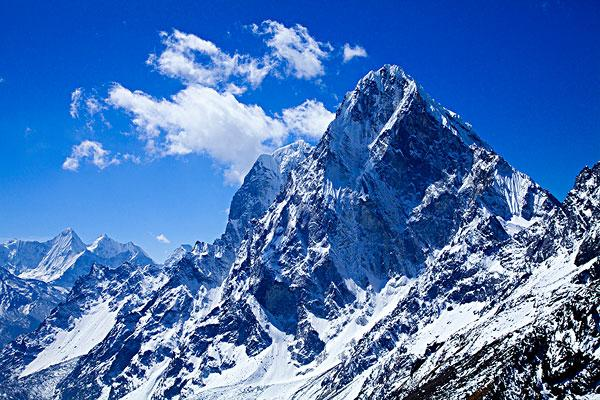
\includegraphics[scale=0.2]{mountain}
        \caption{太白山}\label{fig-mountain}
    \end{figure}



    当然，在\LaTeX{}中也如此使用表\ref{tab-score}所示的表格。

    \begin{table}
        \centering
        \caption{考试信息}\label{tab-score}
        \begin{tabular}{|l|c|c|c|r|}
            \hline
            姓名 & 语文 & 数学 & 外语 & 备注 \\
            \hline
            张三 & 87 & 100 & 93 & 优秀 \\
            \hline
            李四 & 75 & 64 & 52 & 补考另行通知 \\
            \hline
            王二 & 80 & 82 & 78 & 良好 \\
            \hline
        \end{tabular}
    \end{table}
\end{document}
